\pretolerance = 400
`I': it is possibly the most significant signifier in language. It is a
foundational word and a foundational concept---one that determines and
distinguishes an individual, one that creates an identity. Once there is
the `I', by natural law, there is the `not-I', or the `other'. Some
questions then arise: what, if anything, precedes the I/not-I
distinction? What is its nature? What becomes of it after the division
of I/not-I has happened? Can this division ever be undone, and what
would happen if it were undone? Logically, a division is preceded by a
plenum\footnote{Plenum: an absolute wholeness devoid of any breaks or
  gaps.}---here, it must be something that is neither `I' nor `not-I'.
It has long been philosophized that the subject as `I' and the objects
as `not-I' are born of a plenum which is unknown and unknowable, beyond
language and beyond signification.\footnote{The process of indicating or
  naming things in the world by using signs or other symbolic means,
  e.g. words, symbols, etc.} It is entirely ineffable, but it has been
given names throughout history: Spinoza called it `Substantia', Herbert
Spencer the `Unknowable'; it is Kant's \emph{ding an sich}, and
Emerson's `Over-soul'; it is what can be called the Lacanian Real and
the Vedantic Brahman. This paper shall explore the concepts of the Self
and identity as developed in Lacanian psychoanalysis and Advaita
Vedanta; provide a consideration of the ineffable Reality as
conceptualized through Lacan's register of the Real and the ancient
Upanishads' Brahman by showing how both signify a Reality that
transcends and simultaneously pervades the experience of the world; and
discuss whether that Reality is attainable or irretrievably lost.

Before beginning a comparative discussion of the ideas of Jacques Lacan
and the Vedanta with respect to their respective philosophies about the
nature of the Self and identity, a brief account of the Lacanian theory
of psychological registers is provided in the following paragraphs:

According to Lacan, the three psychological registers---namely, the
Real, the Imaginary, and the Symbolic---are what build and comprise the
entire human identity.\footnote{Identity as `I' with a particular
  narrative.} It is in and through these three registers that one
creates, establishes, and maintains one's identity throughout the
lifetime. The Real is a complex and ineffable sense of wholeness that is
carried over into the neonatal state from the foetal state\footnote{Felluga
2011.} It is the experience that one has until about six months of age.
This period is characterized by an undifferentiated experience of the
world: the child does not ``identify'' itself as anything and cannot
differentiate between itself and the world. The world is not experienced
as comprising distinct and distinguishable objects within which the
child is another limited body amongst many. The child has no ability to
distinguish the boundaries between objects for it cannot sense:
``\emph{This} is a table! \emph{That} is a spoon! \emph{This} hand is
\emph{mine}!'' The inability to give separate, identifying names to
different concepts, sensations, or perceptions leaves the child with an
experience of all concepts, sensations, and perceptions as one. As a
result, the experience is one of complete, pure, undifferentiated
wholeness.

This sense of oneness is lost in the Mirror Stage of the Imaginary
Order, the second register, at about six to eighteen months of age.\footnote{Lacan 2008, 76.} It is here that the child recognizes itself in a
mirror and develops the concept of an `I' as well as an identification
of that `I' with the body. It is by consequence of this event that the
Real is irretrievably lost---an irreversible division is created in the
wholeness since now the child is able to identify itself as a distinct
body separate from everything that comprises the `not-I'. This loss of
the Real becomes a haunting lack that torments the established, fictive
`I' for the rest of the lifespan.

The Symbolic Order begins when the individual acquires language, which
further solidifies their created identity. Upon entrance into language,
the mental concept of identity as an `I' is eternally locked through
signification. Having a signifying sign---the word `I'---for the
concept of self as a distinct and contained body permanently solidifies
the conception. Therefore, identity as `I' is entirely contingent upon
language since it is through the linguistic signifier (in English, it is
`I'; in French, `Je'; in Hindi, `\emph{Main}') that the conception of
self as distinct and separate is stabilized. Language is what enables
the identity as `I' to develop a concrete form---`I' becomes a tangible
linguistic position.\footnote{Felluga 2011.} However, the loss (lack) of the Real
is an underlying decisive factor for the movements of the identity
functioning in the Symbolic Order, that is, in the period of life post
language acquisition. Language, Lacan describes, is a surrogate for the
Real, but does not provide the fulfilment of the wholeness of the Real.\footnote{Johnston 2018, 5--6.} The lack of the Real gives rise to an endless
desire---material, sexual, or otherwise---through which the fictive
`I' tries to repair the sense of alienation initiated in the Mirror
Stage. The sense of the lack, the separation, can be overcome by the
loss of the fictive `I', and Lacan theorizes that such a loss can be
obtained only through sex\footnote{Lacan describes the moment of orgasm
  as \emph{jouissance} and \emph{le petit mort}---a short moment of
  ego-death caused due to the satisfaction attained by sexual pleasure.
  Lacan holds this \emph{jouissance} to be greater than simple bodily
  pleasure, it is an acceptance of death. The subject, by submitting
  themselves to the Symbolic Order of language, sacrifices some
  \emph{jouissance,} since ``\emph{jouissance} is forbidden to him who
  speaks''. The moment of orgasm is a short, temporary and
  incomplete experience of \emph{jouissance,} according to Lacan, and
  which is the object of desire that is never attainable and therefore,
  it perpetuates desire.} (the moment of the orgasm) and death.\footnote{Evans
2003, 93.}

Returning, now, to the subject of the paper, the Mirror Stage is when
the subject identifies, or rather, misidentifies
(\emph{méconnaissance}), the \emph{imago-Gestalt}\footnote{\emph{Imago}
  means ``image'' and \emph{Gestalt} refers to the perception of a form
  whose meaning is greater than the sum of its parts, that is, the
  infant recognizes its image in the mirror not only as an assemblage of
  different bodily parts but a meaningful form. For example, the terms
  ``school'' or ``home'' have a meaningful form that is greater than and
  beyond the comprising parts that may be material buildings, people
  (teachers or family), etc.} that is reflected in a mirror as well as
in others' actions, as the `I'.\footnote{Lacan 2008, 76.} Besides being the
causal event for the creation of the I/not-I divide, the Mirror Stage is
also crucial to the creation of the distinction between the true subject
and the ego. In Lacanian philosophy, `the ego, despite conscious senses
to the contrary, is not a locus of autonomous agency, the seat of a
free, true ``I'' determining its own fate'---the ego is distinct from
the subject: it is an object; that is, the `I' is not the true subject,
rather there is a true subject that perceives the fictive `I' as the
self.\footnote{Johnston 2018, 8.} However, there is a period in infancy when the
child---lacking the recognition and linguistic signification of itself
as `I', a distinct body---is pure subject. That is the stage of the
Real: `Lacan tends to speak of the Real as an absolute fullness, a pure
plenum devoid of the negativities of absences, antagonisms, gaps, lacks,
splits, etc.' \footnote{Johnston 2018, 7.} In this period, as aforementioned, the
child has no sense of the `I', and consequently, no sense of the
`not-I'. Lacan characterizes this as a period of wholeness---the pure
subject sees no distinction between itself and the world because it has
neither the concept of `itself' nor of `distinction'. The Mirror Stage
facilitates the idea of identity with the body. Identification of the
ego with the body determines the limitation of the `I' and establishes
all that is `not-body' as `not-I'. What should happen to identity in the
absence of the body? If identity is contingent on the body, should one
assume that what precedes identity is also contingent on the body? It is
known that the body disintegrates after death, and it is unknown what
death truly means. However, one can hypothesize certain possibilities:

\begin{enumerate}
	\item Death is an end of the body as well as the subject, in which case it
is plausible that the subject and the body do share an identity fact.

	\item Death is an end of the body; however, if Lacan's distinction of the
subject and ego is true, and if it is the ego-as-object that identifies
with the body, then the end of the body suggests the end of the
ego-as-object. What, then, are the whereabouts of the subject? If the
subject precedes identity, and if it is distinct from the body, then it
should be possible for the subject to exist even in the absence of
identity and the absence of the body.
\end{enumerate}

This latter possibility recalls Cartesian dualism: the subject and the
body are distinct, separable, and of entirely different natures.
Presently, we are going to assume this substance dualism. Upholding this
dualism, and holding time as a constant, we shall consider this diagram:
\begin{center}
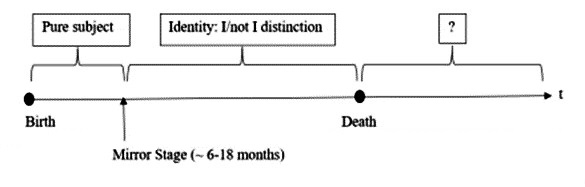
\includegraphics[scale = 0.45]{nathdiagram}
\end{center}
Here,
during the lifetime of the body, the period until the Mirror Stage is
characterized by a lack of identity with the body. Despite the body, the child is pure subject.
This is the period of the Lacanian register of the Real. The Mirror
Stage onwards, there is a misrecognition of the `I' as the ego and the
body, and the I/not-I distinction is created. However, this scenario
assumes the origin of the body (at birth) to be the origin of the
subject, which would imply that the subject is somehow still causally
contingent upon the body. This again raises the question of the
subject's existence independent of the body, i.e. after death. Let us
consider another scenario where the subject, entirely independent of the
body, can precede, and therefore succeed, the body, thereby creating a
timeline such as this:
\begin{center}
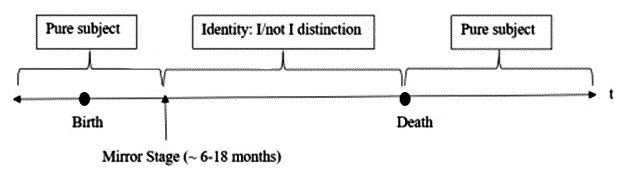
\includegraphics[scale = 0.45]{nathdiagram2}
\end{center}
In this case, the subject exists in time before and after the lifespan
of the body. If the subject and the body are indeed of a substance
dualism, then it can be said that the physical substance of the body
exists for a temporary period in the span of existence of the
non-physical subject. In both the aforementioned scenarios, time has been taken as an external
constant within which the physical body and non-physical subject exist.

In the second scenario, the subject exists indefinitely in both
directions of the timeline. This brings us to the question: What is it
to exist? Is it an experience of time? Does existence necessitate time?
Is `I exist' an experience of a progressing present moment wherein there
is a present in which I am, a past in which I just had been, and a
future in which I will just be? Clearly, this contingence of the
experience of existence upon time is predicated on the fact that there
is a concept of an `I' and that there is a faculty that enables
experience. What happens to existence when there is no concept of an
`I', and no faculty that enables the experience of existence? How can we
say that the `subject exists in time before and after the lifespan of
the body' if it has no concept of an `I' and no body that enables
experience?

On a tangent whose relevance will soon become clear, there arises
another question: if existence is dependent on time, what does it mean,
then, to say that time exists? Does time require an experience of time
in order to exist? Classical physics would consider it unlikely that the
existence of time is dependent on an experience of time (although
according to the theory of special relativity, time is not an absolute---it is something that
exists, the experience of which is relative and flexible). Irrespective
of how it is experienced, both physics and common sense will say: time
\emph{is}. Therefore, if time is an independent entity whose existence
does not depend on any experience of existence, and if the subject can
exist without facilities that enable an experience of existence, then
the subject, like time, is an independent entity whose existence does
not depend on any experience of existence. With this in mind, one can
propose a rather audacious third scenario:
\begin{center}
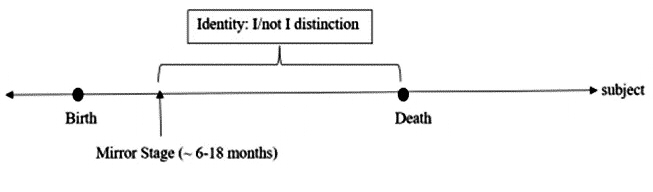
\includegraphics[scale = 0.45]{nathdiagram3}
\end{center}
Here,
the only absolute existence is of the subject. The subject does not
exist \emph{in} time. The subject does not \emph{experience} time. The
subject \emph{is}. The existence of the subject is not dependent on
anything; the subject does not derive its existence from any source.
Entirely self-sufficient, it exists as an absolute, independent
substance. What Lacan calls the Real is the neonatal experience as pure
subject which precedes the Mirror Stage. From the aforementioned
argument about the consequences of death for the subject, the identity,
and the body, we have shown that upon holding Lacan's identity
philosophy true, the existence of the subject can be concluded as
absolute. The Lacanian Real is, in fact, the absolute subject.

A substance duality had been assumed previously which was based on time
as an `external constant within which the physical body and non-physical
subject exist'. Now, since the subject has been shown to be the only
absolute, time is no longer an external constant. The absoluteness of
the subject, therefore, negates substance dualism. There can only be
one, non-dual substance---that of the subject.

It is this non-duality that is the central philosophy of Advaita
Vedanta. The pure subject, the absolute non-dual substance, is termed
`Brahman' in the Upanishads. Adi \'Sa\.nkar\=ac\=arya, the ancient Indian
scholar, summarized the entire philosophy of Advaita in a sentence:
`Brahman is real, the world is an illusion, the self is Brahman itself
and not different' (\'Sa\.nkar\=ac\=arya). The following is the line from his
work \emph{Brahma Jnanavali Mala}:
\begin{center}
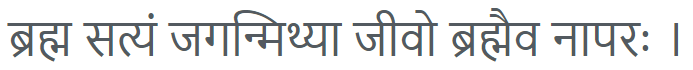
\includegraphics[scale = 0.525]{nathBrahma}

\emph{Brahma satyam jaganmithya jivo brahmaiva naparah}
\end{center}
Brahman, the non-dual reality, the `Ultimate Truth', is defined as
\emph{Satyam Jnanam Anantam,} or infinite existence and consciousness.\footnote{\'Sa\.nkar\=ac\=arya 1995.} It is indescribable and ineffable; `one without a
second', it is beyond language, speech, and mind: `The Absolute
Substance or Brahman is beyond space and time, consequently it is
formless and unchangeable\ldots\ it is our true Self'\footnote{Abhed\=ananda
1992.} The Katha Upanishad mentions: `The all-knowing Self was never
born, nor will it die. Beyond cause and effect, this Self is eternal and
immutable. When the body dies, the Self does not die'.\footnote{\'Sa\.nkar\=ac\=arya
1987.} According to Advaita Vedanta, Brahman is the Self (\emph{Aham
Brahmasmi})---the subject---and the sole absolute substance of the
universe: one cannot say it `exists', for it is existence itself. It is
pure existence and pure consciousness: `Consciousness can never be the
object of knowledge. It is always the subject'.\footnote{Abhed\=ananda 1992.}
Therefore, it can be said that Brahman is the same as the absolute
subject previously described.

What both Brahman and the Real seem to signify is a pure,
undifferentiated subject which is `without fissure' and which `resists
symbolization absolutely'.\footnote{Fink 1997, 24; Lacan 1988, 66.} It is an
absolute wholeness or oneness that precedes the Lacanian Mirror Stage
when the subject misidentifies itself as an object: `I', and
consequently divides the plenum into the `I' and the `not-I'. The true
subject is neither `I' nor `not-I'. Vedanta conveys this through the
concept of \emph{neti-neti} (`not this, not this'). It mentions that the
subject is not the `I' and not the `not-I'; however, the subject is that
within which the `I' and the `not-I' arise. Similarly, one can say that
as the Real underlies the realm of reality as constituted by the
Imaginary and the Symbolic Orders---the `I' and the `not-I' of the
Imaginary and Symbolic Orders arise within the Real, i.e. the absolute
subject.

What happens to the pure subject---the Real or Brahman---once identity
is established in the Mirror Stage? Lacan and Advaita Vedanta provide
slightly different answers. According to Lacan, the Real is
irretrievably lost upon entrance into language. The Real is entirely
beyond language: the very signification of it as `Real'---a word in
language---marks our irrevocable separation from it. Lacan would hold
that its signification---as the `Real' or as `Brahman'---makes it
eternally elusive. However, Lacan mentions that the Real, underlying the
realm of the Symbolic and Imaginary, can appear to erupt in guises of
```limit experiences'', namely, encounters with that which is
annihilating, inassimilable, overwhelming, traumatic, or unbearable'.\footnote{Johnston 2018, 13.}

The eruption of the Real is fleeting and incomplete, either pleasurable
(for example, at the moment of orgasm) or traumatic in case of events
that cause the experience of the world to become gravely shaken. In
Seminar XI, he mentions: `Is it not remarkable that, at the origin of
the analytic experience, the real should have presented itself in the
form of that which is \emph{unassimilable} in it-in the form of the
trauma, determining all that follows, and imposing on it an apparently
accidental origin?'\footnote{Lacan 2005, 55.} When the fabric of the Symbolic is
ruptured, the Real seemingly erupts, and it is perceived as traumatic
because it threatens the known and consolidated reality of the `I' and
the `not-I'. Despite that annihilation of the fictive `I' being the very
object of desire, the threatening nature of that destruction and the
fear that it evokes in the individual is the same as the fear of death
and the unknown that lies beyond. Therefore, the individual remains in a
lifelong struggle between desiring and fearing that where the `I' and
the `not-I' are no longer separate, where language and signification no
longer exist; that which is unknown and unknowable; that which is beyond
death.

Advaita Vedanta, however, states that Brahman is never lost---it is
ever present---but we do not realize it due to ignorance\emph{:
`}Though the Self is Brahman, there is not the knowledge of the Self
(being Brahman). That which obstructs the knowledge of the Self is
Ignorance.'\footnote{Harihar\=ananda 2002.} According to the scriptures, Brahman
can be realized primarily through the practice of focused and meditative
\emph{vic\=ara} (discrimination) which allows one to discriminate between
what is truly the Self and what is not.\footnote{Dhire\'s\=ananda 2014.}
Brahman is beyond language, but it can be realized despite language, and
also through language: `\emph{Aum,} the word, is all this\ldots\
\emph{Aum} is the means to the knowledge of Brahman on account of its
having the closest proximity to Brahman'.\footnote{\'Sa\.nkar\=ac\=arya 1995.}

Is it possible to regain the Real or realize Brahman in the lifetime of
the body, once again like the neonatal pure subject? Can the
misidentification of the subject as the object `I', and the subsequent
I/not-I division, be reversed? Can identity ever truly be lost? Is the
ineffable really irretrievably lost when we enter into language, as
Lacan states? Is the only way to enter the state of pure subject once
again (while having the body and sense perceptions, i.e. before death)
to lose language? Let us introduce a thought experiment to consider the
possibilities: Soham is an adult who has lost all their acquired
knowledge of language. Their severe aphasia is a result of acute and
irreversible cerebral damage. Not only are their Broca's and Wernicke's
areas for language production and comprehension in the brain completely
damaged but also their entire store of knowledge and memories of ever
having learnt language has been erased. They are now exactly how they
had been before being introduced into language. However, they still
retain their sense perceptions which allow them to perceive the world
just as before; but the world has no meaning to them since they have no
way of signifying their perceptions such that one perception is
differentiated from another. Now, what should be the impact of this
severe loss on their identity?

Identity, besides being a sense of an `I', is certainly dependent on
memory: the knowledge and events that provide a history to the `I'. The
erasure of all knowledge of language can have a severe impact on Soham's
memories, especially semantic and episodic. It is implausible that
without a process of signification that would allow them to
differentiate perceptions (even memories of past perceptions), Soham
retains the normal memory functions. Therefore, due to Soham's inability
to signify and differentiate objects, their memories can become entirely
redundant. This will have a severe impact on their identity as Soham.
The effect of losing memories on a person's identity is evidenced by
real cases of severe dissociative amnesia; therefore, Soham's
autobiographical identity should, as a result of losing memory function,
also be lost. Having lost a major portion of what defines his identity,
the question now is whether they retain the sense of an `I'.

One possibility is this: since the Mirror Stage appears to precede
entrance into language, it is possible that Soham entirely retains the
sense of identity with the body. The loss of language has no effect on
the consequences of the Mirror Stage they experienced as a child.
Therefore, they are still aware of their bodily integrity. Furthermore,
the loss of language will not hamper their ability to still recognize
their body in a mirror. However, one can be skeptical of this
possibility: how do they identify themselves if they do not have the
faculty of signification? Without any faculty of signification or
learning signification (they do not comprehend when others tell them
that what they see is a mirror, and that the mirror reflects, and that
what they see in the mirror is themselves) seeing themselves in a mirror
would make no sense to them---it would be just another perception that
cannot be signified and differentiated. Still, one can argue that the
effects of the Mirror Stage remain from the memory of the childhood
experience; however, since the loss of language can render episodic
memories redundant, it is unlikely that the memory of the childhood
event will have any consequences on present-day Soham. This scenario,
therefore, is quite unconvincing.

Here, second possibility can be considered. Although Lacan's text of
`The Mirror Stage' seems to suggest that the Imaginary Order precedes
the Symbolic Order, his later emphasis on the role of other human beings
in the process of identification with the \emph{imago-Gestalt} suggests
that the effects of the Imaginary and Symbolic registers occur
simultaneously. The Mirror Stage of the Imaginary Order cannot be
considered to be an event that occurs outside of the influence of
language:
\begin{quote}
if anything, socio-linguistic variables (for instance, the words and
body language of parents) are the causal triggers of the child's
investment in select sensory-perceptual experiences (such as the body
image in the mirror)\ldots{} this means that the imagistic nucleus of
the ego is suffused from the get-go with the destinal ``discourse of the
Other''--- in this case, fateful significations (``unary traits'')
coming from caregivers' narratives articulated simultaneously along with
their encouragements to the child to recognize him/her-self in the
mirror.\footnote{Johnston 2018, 9.}
\end{quote}
It is extremely important to consider that `socio-linguistic
variables\ldots\ are the causal triggers of the child's investment in
select sensory-perceptual experiences (such as the body image in the
mirror)'.\footnote{Johnston 2018, 9.} If language is the very `causal trigger'
for the Mirror Stage, then with their redundant memories and inability
to signify anymore, Soham can be said to have reverted from the
consequences of the Mirror Stage. Not only have they reverted but also
cannot undergo the Mirror Stage event again because the very `causal
trigger' has been taken away. Can it be said, then, that they no longer
have any sense of an `I'? Has the I/not-I divide now been reversed? Is
Soham now purely the absolute subject, despite retaining their body? It
is plausible that through this extreme separation from the Symbolic,
Soham reverts from the effects of the Mirror Stage and Imaginary Order
and resists undergoing the same effects again. With the Symbolic and the
Imaginary removed entirely, only the Real remains. And, Soham has
regained the Real---they are pure subject.

This thought experiment considered the Lacanian view, and it appears
that language is indeed the fundamental factor that determines identity.
The Self as the Real---or Brahman---cannot be regained as long as one
remains in language. The Self shall remain entirely out of reach unless
a person is subject to a loss of language as radical as Soham's. Lacan
points out this elusiveness of the Self due to the established identity
and the faculties of signification in \emph{\'Ecrits:} `I think where I am
not, therefore I am where I do not think. I am not whenever I am the
plaything of my thought; I think of what I am where I do not think to
think'.\footnote{Lacan 2008, 166.} If language binds us in identity, how does one
undo the I/not-I divide and return to the state of pure subject,
according to the Upanishads? Advaita Vedanta advocates for the
realization of the Self as Brahman---pure, non-dual subject---through
the \emph{jnana yoga}, or the way of knowledge. Through knowledge and
rational \emph{vic\=ara}\footnote{Discrimination.}, one can realize the
true nature of the Self. The ancient text of the \emph{Yogav\=asi\d s\d tas\=ara\d h}
mentions:
\begin{quote}
The firm immediate knowledge of the Self arises due to discrimination
by means of \emph{manana}\footnote{Intellectual reflection.} and
\emph{nididhy\=asana}\footnote{Internal contemplation.}\ldots\ By that
discrimination the veil, which causes non perception of Brahman and the
projection, or the reflected consciousness with gross and subtle bodies
and their properties\ldots{} gets obscured and that leads to liberation.
People have their strong ego-identities in their bodies; if such a
strong ego-identity in Brahman comes and obstructs the body-identity, it
is called \emph{immediate} (\emph{aparok\d sa}) and unmoving direct
Knowledge of Brahman.\footnote{Dhire\'s\=ananda 2014.}
\end{quote}
This excerpt suggests that the identity that one feels with one's body
can be replaced by an `ego identity in Brahman'. One can realize this
through wisdom and earnest reflection upon the \emph{vic\=ara} which
allows one to see that the apparent world is not the true Reality.
Focused meditation on the `unreal' nature of the world allows one to
realize that the I/not-I divide is an illusion, and that the Ultimate
Truth is Brahman\footnote{\'Sa\.nkar\=ac\=arya 1995.} The \emph{Yogav\=asi\d s\d tas\=ara\d h}
continues to say that the \emph{jīvanmukta}'s (liberated person) `unreal
worldly behaviors continue, with the help of the false body, senses and
the like' due to his material body.\footnote{Dhire\'s\=ananda 2014.} He continues to
live as he did before his knowledge of the Self as Brahman; however, he
no longer identifies himself as his body---he is aware of the fact that
the `I' and the `not-I' are unreal.

In the \emph{Four Fundamental Concepts of Psychoanalysis}, Lacan
mentions: `it is the subject who introduces division in the individual
{[}habit of saying I{]}, as well as into the collectivity that is his
equivalent {[}others{]}. Psychoanalysis is properly that which reveals
both the one and the other to be no more than mirages'.\footnote{Lacan 2005, 80.}
Vedanta calls `illusion' precisely what Lacan calls `mirages'. What
Lacan says psychoanalysis reveals is precisely what Vedanta says is
revealed through the \emph{jnana yoga}. However, does the knowledge of
Brahman equate to the true experience of Brahman? Is knowledge of the
Real equal to true experience of the Real? Is knowing of the falsity of
the I/not-I divide equivalent to undoing the division?

It appears that realization through knowledge and realization through
experience (like Soham's) are quite different. In the former mode of
realization, one recognizes the I/not-I divide to be unreal but
continues to remain and function in the world without the actual
experience of pure subject. The latter realization is difficult to be
termed as a realization since that would require the ability to compare,
which further requires the faculty of signification. The pure subject
experience of Soham comes at the cost of complete impairment of
functioning in the world. The body becomes irrelevant to Soham;
therefore, the presence or absence of the body should not affect Soham's
state as pure subject. Soham's state before body-death is exactly the
same as their state post body-death. One can say that what they have
achieved in life is precisely what they would have achieved in death.
The knowledge of Brahman---or the Real---entails that one identifies
oneself as Brahman: this can be quite superficial in comparison to the
actual experience as pure subject (like Soham's). To say that one
identifies oneself \emph{as} something, is to employ the faculties of
signification. To say that one identifies as Brahman or the pure subject
is a consolidation of the `I' and the `not-I', not an eradication of the
`I' and the `not-I'---which is what is necessary in order to regain the
Real.

There is much that can be said about the philosophies which speak of the
ineffable plenum---call it Brahman or the Real---which is the  Ultimate
Truth, and that very endless discourse is what makes it elusive. It
escapes us for as long as we can think of it, and it embraces us the
very moment we escape thought. Perhaps, as Lacan and the Vedanta have
said, as long as we have the faculties of signification and the body, we
can only reach as far as knowing that there is something beyond the
illusion of the `I' and the `not-I', and that the Self is greater than
what the ego and the body suggest it to be. Perhaps, it is with
knowledge, that is the consolidation of the `I' and the `not-I', that
one should live numerous peaceful years, and it is in anticipation of
the complete dissolution of the `I' and the `not-I', that one should
welcome death.

\clearpage
\section*{References}
{
\small
\begin{itemize}[label={},itemindent=-2em,leftmargin=2em]	
	\item Abhed\=ananda. \emph{Self-Knowledge}. Ramakrishna Vedanta Math, 1992.


	\item Dhire\'s\=ananda and Sarvadev\=ananda. \emph{Yogav\=asi\d s\d tas\=ara\d h}. Sri
Ramakrishna Math, 2014.


	\item Evans, Dylan. \emph{An Introductory Dictionary of Lacanian
Psychoanalysis}. {Hove: Brunner-Routledge}, 2003.


	\item Felluga, Dino F\emph{.} ``Modules on Lacan: On the Structure of the
Psyche.'' \emph{Introductory Guide to Critical Theory.} Purdue University, January 31, 2011.

	\item Fink, Bruce. \emph{The Lacanian Subject: between Language and
Jouissance}. Princeton University Press, 1997.

	\item Harihar\=ananda, Sarasvat\=i. \emph{Advaita Bodha Deepika, the Lamp of
Non-Dual Knowledge}. Sri Ramanasramam, 2002.

	\item Johnston, Adrian. ``Jacques Lacan.'' Stanford Encyclopedia of
Philosophy. Stanford University, July 10, 2018.

	\item Lacan, Jacques, and Jacques-Alain Miller. \emph{The Seminar of Jacques
Lacan}. Norton, 1988.

	\item Lacan, Jacques, et al. \emph{The Four Fundamental Concepts of
Psychoanalysis}. W. W. Norton \& Company, 2005.

	\item Lacan, Jacques, et al. \emph{\'Ecrits: a Selection}. Routledge, 2008.

	\item \'Sa\.nkar\=ac\=arya, Acarya, Gaudapada,. \emph{The Mandukya Upanishad: with the
Karika of Gaudapada, and the Commentary of Sankaracarya}. Advaita Ashrama,
1995.

	\item \'Sa\.nkar\=ac\=arya. \emph{Katha Upanishad}. Advaita Ashrama, 1987.
	
\end{itemize}
}